\documentclass[10pt,a4paper]{article}
\usepackage[T1]{fontenc}
\usepackage{lmodern,microtype}
\usepackage{amsmath,amssymb,amsthm,mathtools,booktabs,geometry,xcolor}
\usepackage[hidelinks]{hyperref}
\usepackage{tikz}
\usepackage{enumitem}
\geometry{margin=24mm}
\setlist[itemize]{leftmargin=1.8em,itemsep=2pt}
\newtheorem{theorem}{Theorem}[section]
\newtheorem{lemma}[theorem]{Lemma}
\newtheorem{proposition}[theorem]{Proposition}
\newtheorem{remark}[theorem]{Remark}
\newcommand{\Rcrit}{R_0}
\newcommand{\Rcap}{U}
\newcommand{\radii}{\{3,4,5,6,7,8\}}
\newcommand{\dist}[1]{\lVert #1\rVert}
\newcommand{\Q}{\mathbb Q}
\title{Certified Global Optimality for Packing Eight Disks\\of Radii $1,2,\ldots,8$ in a Circle}
\author{Computer-assisted proof note --- verification draft}
\date{9 October 2026}
\begin{document}
\maketitle
\begin{abstract}
We give a computer-assisted proof of the exact minimum circular-container radius for disks of radii $1,2,\ldots,8$. The optimum $R_0\in(16.22174667655772,16.22174667655773)$ is the unique root of an explicit six-angle closure equation. The lower bound already follows from disks $3,\ldots,8$: a rational radial subdivision with 53 nodes exhausts their 60 cyclic orders, using angular negative cycles at 26 leaves and a radial monotonicity barrier at the remaining leaf. An exact eight-disk realization gives the matching upper bound. All certificate decisions are replayed using integer and rational arithmetic; the proof is not a formal verification in a theorem prover.
\end{abstract}

\section{The exact optimum and its contact equation}
For each $i=1,\ldots,8$, let the disk of radius $i$ have center $p_i\in\mathbb R^2$. A packing in a circular container of radius $R$ satisfies
\begin{equation}\label{eq:packing}
 \dist{p_i}+i\le R,\qquad \dist{p_i-p_j}\ge i+j \quad(i\ne j).
\end{equation}
Put $s_i=\dist{p_i}$. The candidate configuration has a six-disk outer ring in cyclic order
\begin{equation}\label{eq:core}
 \mathcal C=(4,8,3,6,5,7),\qquad
 E_{\mathcal C}=\{(4,8),(8,3),(3,6),(6,5),(5,7),(7,4)\}.
\end{equation}
For two disks touching the container, their necessary central angle at mutual contact is
\begin{equation}\label{eq:beta}
 \beta_{ij}(R)=2\arcsin\sqrt{\frac{ij}{(R-i)(R-j)}}
 \qquad (R>i+j).
\end{equation}
Define the six-angle sum
\begin{equation}\label{eq:closure}
 \Phi(R)=\sum_{(i,j)\in E_{\mathcal C}}\beta_{ij}(R),\qquad
 \Phi(\Rcrit)=2\pi.
\end{equation}
Each $\beta_{ij}$ is continuous and strictly decreasing in $R$ on the interval of interest. Exact rational interval evaluations certify
\begin{equation}\label{eq:bracket}
 \Phi(16.22174667655772)>2\pi,\quad
 \Phi(16.22174667655773)<2\pi.
\end{equation}
Thus Equation~\eqref{eq:closure} defines a unique root
\[
16.22174667655772<\Rcrit<16.22174667655773.
\]
The decimals in this paper denote exact rationals when used as interval endpoints or certificate values.

\begin{theorem}[Exact global optimality]\label{thm:main}
For eight nonoverlapping disks with radii $1,2,\ldots,8$, the minimum radius of a containing circle is the exact number $\Rcrit$ defined in \eqref{eq:closure}. In particular, there is an eight-disk packing at $R=\Rcrit$, but no such packing at $R<\Rcrit$.
\end{theorem}
We prove the upper bound first, then exclude every smaller radius using the six largest disks.

\section{An exact eight-disk realization}\label{sec:upper}
At $R=\Rcrit$, place disk $4$ at $(\Rcrit-4,0)$. For the cyclic order \eqref{eq:core}, define
\begin{equation}\label{eq:centers}
 p_i=(\Rcrit-i)(\cos\theta_i,\sin\theta_i),\quad
 \theta_4=0,\quad
 \theta_{\mathcal C_{k+1}}=\theta_{\mathcal C_k}+\beta_{\mathcal C_k,\mathcal C_{k+1}}(\Rcrit).
\end{equation}
The first five successive pairs are tangent by the cosine law, and the last pair $(7,4)$ is tangent by the closing equation $\Phi(\Rcrit)=2\pi$. All six centers are on the container wall. For the two remaining disks use the rational coordinates
\begin{equation}\label{eq:small}
 \boxed{p_1=(-3,-14),\qquad p_2=(-3,-5/2).}
\end{equation}
A rational interval verifier encloses $\Rcrit$, every rotation cosine and sine in \eqref{eq:centers}, and all resultant center coordinates. It proves strict separation for all $\binom82-6=22$ noncontact pairs and strict containment for disks $1$ and $2$. In particular, it certifies the squared inequalities
\[
 \dist{p_i-p_j}^2-(i+j)^2>0 \quad\text{for every noncontact pair},
 \qquad (\Rcrit-i)^2-\dist{p_i}^2>0 \quad (i=1,2).
\]
The six listed contact equalities follow symbolically from \eqref{eq:closure}. Hence the packing exists at the exact root: $R^*\le\Rcrit$.

\begin{figure}[htbp]\centering
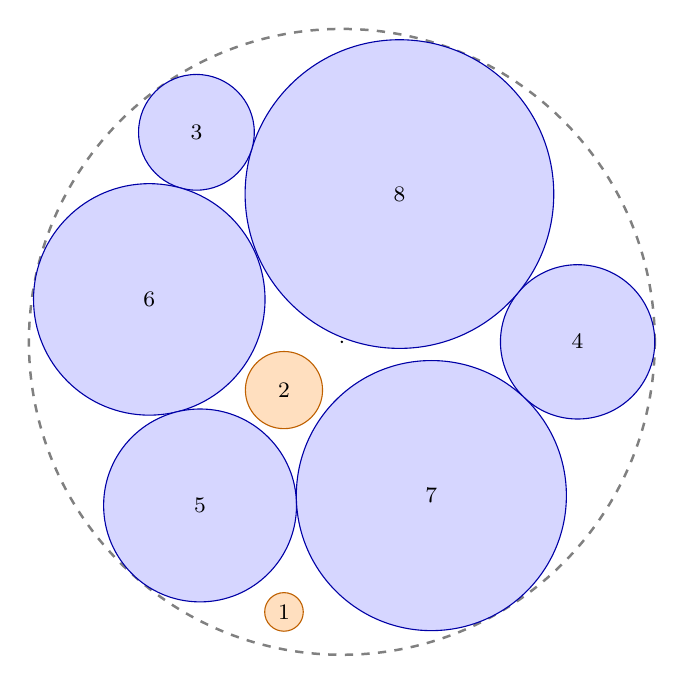
\begin{tikzpicture}[scale=.245, every node/.style={font=\footnotesize}]
  \draw[gray,dashed,line width=.9pt] (0,0) circle (16.221747);
  \draw[fill=blue!16,draw=blue!65!black] (12.221747,0) circle (4);
  \draw[fill=blue!16,draw=blue!65!black] (2.985179,7.660667) circle (8);
  \draw[fill=blue!16,draw=blue!65!black] (-7.538674,10.861997) circle (3);
  \draw[fill=blue!16,draw=blue!65!black] (-9.982178,2.200052) circle (6);
  \draw[fill=blue!16,draw=blue!65!black] (-7.349378,-8.480227) circle (5);
  \draw[fill=blue!16,draw=blue!65!black] (4.639750,-7.969525) circle (7);
  \draw[fill=orange!25,draw=orange!75!black] (-3,-14) circle (1);
  \draw[fill=orange!25,draw=orange!75!black] (-3,-2.5) circle (2);
  \foreach \i/\x/\y in {4/12.221747/0,8/2.985179/7.660667,3/-7.538674/10.861997,6/-9.982178/2.200052,5/-7.349378/-8.480227,7/4.639750/-7.969525,1/-3/-14,2/-3/-2.5}
    \node at (\x,\y) {$\i$};
  \fill (0,0) circle (2pt);
\end{tikzpicture}
\caption{An illustrative drawing of the exact eight-disk witness. Blue disks comprise the six-disk tangent ring; orange disks have rational centers. Rounded coordinates are used for the drawing only, not for proof decisions.}
\label{fig:packing}
\end{figure}

\section{Exact angular inequalities on radial rectangles}\label{sec:generic}
Assume for contradiction that a packing exists with $R<\Rcrit$. It is contained in the rational cap
\begin{equation}\label{eq:U}
 \Rcap=16.22174667656>\Rcrit.
\end{equation}
The six center radii $s_i$ for $i\in\radii$ satisfy
\begin{equation}\label{eq:box}
 \ell_i:=\max\bigl(0,\max_{1\le j\le8,\,j\ne i}(i+2j-\Rcap)\bigr)
 \le s_i\le u_i:=\Rcap-i.
\end{equation}
Indeed, $i+j\le\dist{p_i-p_j}\le s_i+s_j\le s_i+(\Rcap-j)$. The six lower endpoints $\ell_i$ are strictly positive, so their center directions are defined.

For two disks with positive center radii $x,y$, put
\begin{equation}\label{eq:cosphi}
 c_{ij}(x,y)=\frac{x^2+y^2-(i+j)^2}{2xy},\qquad
 \phi_{ij}(x,y)=\arccos c_{ij}(x,y)
\end{equation}
whenever the latter is defined. The cosine law and nonoverlap force the smaller central angle to be at least $\phi_{ij}$. Consequently, in a counterclockwise cyclic order of center directions, each directed angular gap between two consecutive selected disks is at least their necessary smaller angle.

\begin{lemma}[Four-corner cosine bound]\label{lem:corners}
For $d>0$, the function $c_d(x,y)=(x^2+y^2-d^2)/(2xy)$ attains its maximum on any positive rectangular domain at one of its four corners.
\end{lemma}
\begin{proof}
For fixed $y>0$,
\[
\frac{\partial c_d}{\partial x}=\frac{x^2-y^2+d^2}{2yx^2}.
\]
As $x$ increases, the numerator strictly increases, so an interior stationary point, if any, is a minimum. Thus the $x$-maximum lies at an endpoint. Applying the same argument in $y$ on these two edges establishes the claim.
\end{proof}

\begin{lemma}[Certified angular ticks]\label{lem:ticks}
Let $B$ be a positive radial box and $q_{ij}\in\Q\cap[0,\pi]$. Suppose the rational Taylor polynomial
\[
 C_{18}(q)=\sum_{k=0}^{9}\frac{(-1)^kq^{2k}}{(2k)!}
\]
satisfies
\begin{equation}\label{eq:tickproof}
 C_{18}(q_{ij})\ge
 \max_{x\in\{\ell_i,u_i\},\,y\in\{\ell_j,u_j\}}c_{ij}(x,y).
\end{equation}
Then every feasible packing whose radial vector lies in $B$ has pairwise smaller central angle at least $q_{ij}$.
\end{lemma}
\begin{proof}
For $q\in[0,\pi]$, the alternating Taylor remainder gives $\cos q\ge C_{18}(q)$. Lemma~\ref{lem:corners} bounds the radial cosine by the right-hand side of \eqref{eq:tickproof}. For an actual nonoverlapping pair, $c_{ij}(s_i,s_j)\le\cos q_{ij}$, so monotonicity of cosine on $[0,\pi]$ yields the assertion.
\end{proof}

For a lifted cyclic order $(i_0,\ldots,i_5)$, let
$\theta_0\le\cdots\le\theta_5<\theta_0+2\pi$ be the center directions.
Any certified pair tick, including nonadjacent pairs, gives
\begin{equation}\label{eq:diff}
 q_{i_ai_b}\le\theta_b-\theta_a\le2\pi-q_{i_ai_b}\qquad(0\le a<b\le5).
\end{equation}
The directed inequalities can be written as $\theta_v-\theta_u\le w_{uv}$. Any directed cycle with negative total weight contradicts feasibility, since summing its inequalities yields $0\le\sum w_{uv}<0$.

\section{A complete rational exclusion tree}\label{sec:tree}
The six labeled disk directions have $(6-1)!/2=60$ cyclic orders up to rotation and reflection. The verifier enumerates every representative with disk $8$ first and fixes one of the two mirror orientations.

The proof certificate recursively splits the initial rational box \eqref{eq:box}, propagating the necessary radial pair inequalities $s_i+s_j\ge i+j$. Each split is at a rational interior point, and its two closed children cover the parent domain. At each leaf the verifier uses Lemma~\ref{lem:ticks} and exact difference-constraint graphs to exclude cyclic orders.

For positional indices $a<b$, it encodes \eqref{eq:diff} as the two directed edges
\begin{equation}\label{eq:weights}
 b\longrightarrow a:\ -q_{i_ai_b},\qquad
 a\longrightarrow b:\ 2\pi_+-q_{i_ai_b},
 \quad\pi_+=3.141592653590>\pi.
\end{equation}
The inequality $\pi<\pi_+$ is itself checked with Machin's identity and exact alternating rational arctangent bounds. Each edge weight is rational, and the verifier checks that a recorded negative cycle is indeed a simple directed cycle with the declared weights and strictly negative rational sum.

\begin{proposition}[Exhaustive finite reduction]\label{prop:tree}
A rational 53-node binary certificate covers every center-radius vector compatible with $R\le\Rcap$. Its leaves comprise 26 angular leaves, each certifying a negative cycle for all 60 cyclic orders, and one remaining leaf that certifies negative cycles for 59 orders. The sole unexcluded cyclic order at that last leaf is
\begin{equation}\label{eq:last}
 (8,3,6,5,7,4),
\end{equation}
which is a rotation of the contact ring \eqref{eq:core}.
\end{proposition}
\begin{proof}
The provided checker replays all 26 rational splits and all 27 leaves, verifies parent--child coverage and the radial propagation rules, checks each supplied Taylor angle tick, and recomputes each recorded negative cycle using fractions. It verifies 1,619 order-specific cycles in total. As an example, in one ordinary leaf for order $(8,3,5,7,4,6)$, the positional cycle corresponds to
\[
6\to4\to7\to3\to8\to6.
\]
Its five rational angle ticks are $1.138735,1.379586,1.231977,1.490148,1.713582$; the cycle weight is
\[
 2\pi_+-(1.138735+1.379586+1.231977+1.490148+1.713582)
 =-0.67084269282<0.
\]
Every other leaf/order contradiction is represented by corresponding rational data in the accompanying JSON certificate. The rational replay rejects any unrecorded or inconsistent branch or cycle.
\end{proof}

\begin{table}[htbp]\centering\small
\caption{Size of the replayed finite global certificate.}\label{tab:tree}
\begin{tabular}{lr}\toprule
Recorded nodes & 53\\
Rational splits & 26\\
Leaves & 27\\
Leaves excluding all 60 cyclic orders & 26\\
Final leaves retaining one cyclic order & 1\\
Explicit negative-cycle checks & 1,619\\
Maximum subdivision depth & 23\\
\bottomrule\end{tabular}
\end{table}

\section{Closing the last order by wall-angle monotonicity}\label{sec:barrier}
It remains to exclude the cyclic order \eqref{eq:last} when $R<\Rcrit$.

\begin{lemma}[Radial wall comparison]\label{lem:wall}
Let $i,j$ be disks with center radii in positive intervals
$[\ell_i,u_i]$, $[\ell_j,u_j]$. Suppose throughout the rectangle
\[
 x+y>i+j,\quad |x-y|<i+j,\quad
 x^2-y^2+(i+j)^2>0,\quad y^2-x^2+(i+j)^2>0.
\]
Then $\phi_{ij}(x,y)$ is strictly decreasing in each radial coordinate separately. In particular, if $x\le R-i$ and $y\le R-j$ and the rectangle includes these wall radii, then
\begin{equation}\label{eq:wall}
 \phi_{ij}(x,y)\ge\phi_{ij}(R-i,R-j)=\beta_{ij}(R).
\end{equation}
\end{lemma}
\begin{proof}
Direct differentiation of \eqref{eq:cosphi} gives
\begin{equation}\label{eq:derivative}
 \frac{\partial\phi_{ij}}{\partial x}
 =-\frac{x^2-y^2+(i+j)^2}{2x^2y\sin\phi_{ij}(x,y)}.
\end{equation}
The assumed triangle inequalities ensure $0<\phi_{ij}<\pi$; thus the denominator is positive and the numerator is strictly positive. The corresponding derivative with respect to $y$ is likewise negative. Increase the radial variables in the angle formula one at a time; this is an analytic comparison, not a physical displacement of disks.
\end{proof}

For the last radial leaf, let $\ell'_i$ be its propagated lower endpoints. The exact checker verifies for each adjacent pair $(i,j)\in E_{\mathcal C}$ that the extended rectangle
\[
 [\ell'_i,\Rcap-i]\times[\ell'_j,\Rcap-j]
\]
satisfies the hypotheses of Lemma~\ref{lem:wall}. In particular, it checks the endpoint conditions
\begin{align*}
 \ell'_i+\ell'_j&>i+j,\\
 \max\bigl\{|\ell'_i-(\Rcap-j)|,|\ell'_j-(\Rcap-i)|\bigr\}&<i+j,\\
 (\ell'_i)^2-(\Rcap-j)^2+(i+j)^2&>0,
\end{align*}
and the last inequality with $i$ and $j$ exchanged. Table~\ref{tab:intervals} gives readable decimal displays; all actual checks use the exact rational endpoints in the certificate.

\begin{table}[htbp]\centering\small
\caption{Final barrier-leaf radial ranges (decimal displays, not proof inputs).}\label{tab:intervals}
\begin{tabular}{ccc}\toprule
Disk $i$ & Certified lower endpoint $\ell'_i$ & Upper endpoint $\Rcap-i$\\\midrule
3&12.895387509275&13.221746676560\\
4&11.694028341990&12.221746676560\\
5&10.819028341990&11.221746676560\\
6&9.944028341990&10.221746676560\\
7&8.916310007420&9.221746676560\\
8&7.916310007420&8.221746676560\\
\bottomrule\end{tabular}
\end{table}

Now suppose a packing with $R<\Rcrit$ survives the finite tree. Proposition~\ref{prop:tree} forces the cyclic order \eqref{eq:last} and the last radial box. Lemma~\ref{lem:wall}, applied to all six consecutive pairs, yields
\begin{equation}\label{eq:contradiction}
 \underbrace{2\pi}_{\text{complete turn}}
 \ge\sum_{(i,j)\in E_{\mathcal C}}\phi_{ij}(s_i,s_j)
 \ge\sum_{(i,j)\in E_{\mathcal C}}\beta_{ij}(R)
 >\sum_{(i,j)\in E_{\mathcal C}}\beta_{ij}(\Rcrit)=2\pi.
\end{equation}
The strict inequality follows because $R<\Rcrit$ and each $\beta_{ij}$ is strictly decreasing in $R$. This contradiction proves $R^*\ge\Rcrit$; Section~\ref{sec:upper} established the reverse inequality. Theorem~\ref{thm:main} follows.

\section{Reproducibility and scope}
The verifier files are
\begin{center}
\begin{minipage}{.92\linewidth}\small\ttfamily
certify\_integer\_eight\_global.py\\
verify\_eight\_upper.py\\
verify\_eight\_global\_tree.py\\
eight\_global\_proof\_tree.json
\end{minipage}
\end{center}
Run \texttt{python3 certify\_integer\_eight\_global.py} from their directory with Python 3.11 or newer, without \texttt{-O}/\texttt{-OO}. The root/witness verifier checks rational enclosures of radicals, inverse trigonometric terms, $\pi$, and strict geometric slacks. The global-tree verifier checks all rational split and angle-cycle data and the final monotonicity conditions. Certificate discovery code is not required to replay the results.

\begin{remark}[Trust boundary]
This is a computer-assisted mathematical proof conditional on the soundness of the accompanying verification code and Python's exact integer and \texttt{Fraction} semantics. It is neither an end-to-end Lean formalization nor a claim of independent peer review. The exact value is specified by the isolated transcendental-looking angular closure equation; no minimal polynomial is claimed in this note.
\end{remark}
\end{document}
